\documentclass[11pt]{article}
\usepackage[margin=1in]{geometry}
\usepackage{amsmath,amssymb}
\usepackage{booktabs}
\usepackage{graphicx}
\usepackage{hyperref}
\usepackage{float}

\newcommand{\E}{\mathbb{E}}
\newcommand{\R}{\mathbb{R}}
\newcommand{\TE}{\operatorname{TE}}

\title{Data 37711 Homework 2 --- Problem 2\\
\large Encoding high-cardinality categorical features}
\author{Yiwen Chen}
\date{}

\begin{document}
\maketitle

The code is in \texttt{problem2.py}. All numbers below come from one run with seed 0.

%==========================================================================
\section*{Setup: target transformation and loss}

\texttt{Quantity} is a positive integer with a very heavy right tail:
\[
\text{median}=6,\quad q_{0.9}=24,\quad q_{0.99}=120,\quad q_{0.999}=504,\quad \max=80{,}995,
\]
with mean 13.0 and standard deviation 180. With squared error on the raw scale, a handful of
huge orders would dominate the loss and the gradients. Since $\texttt{Quantity}\ge1$, I instead
model
\[
 t = \log(\texttt{Quantity}) \in [0,\, 11.3],
\]
and train every model with mean squared error on $t$:
\[
 \mathcal L(\theta)=\frac1n\sum_{i=1}^n\bigl(t_i-\hat t_\theta(x_i)\bigr)^2 .
\]
This is the maximum-likelihood loss for the model
$\log Y\mid x\sim\mathcal N(\hat t(x),\sigma^2)$, i.e.\ a log-normal model for
\texttt{Quantity}. Large orders count in relative rather than absolute terms: predicting 60 for
a true value of 120 costs the same as predicting 3 for a true value of 6. The prediction
$\exp(\hat t(x))$ estimates the conditional \emph{median} (geometric mean) of \texttt{Quantity},
which is a sensible point forecast for a skewed target.

\paragraph{Metrics.} On the test set I report RMSE, MAE and $R^2$ on the log scale (the training
objective), and the MAE and median absolute error of $\exp(\hat t)$ in original units.

%==========================================================================
\section*{(a) Cardinality and data split}

\begin{table}[H]\centering
\begin{tabular}{lccccc}
\toprule
Feature & \# unique & rows/level (median) & min & max & levels with $<5$ rows\\
\midrule
\texttt{StockCode}  & 3{,}665 & 49 & 1 & 2{,}035 & 472\\
\texttt{CustomerID} & 4{,}339 & 41 & 1 & 7{,}847 & 228\\
\bottomrule
\end{tabular}
\caption{Cardinality of the two features ($n=397{,}924$ rows; 266{,}802 distinct
(item, customer) pairs).}
\end{table}

Both features have \emph{high cardinality}: thousands of levels, many of them rare. This has
three consequences.
\begin{itemize}
 \item \textbf{One-hot encoding is feasible, but only as a sparse matrix.} It produces
 $3{,}665+4{,}339=8{,}004$ columns. A dense \texttt{float32} design matrix would take
 $397{,}924\times 8{,}004\times4$ bytes $\approx 12.7$\,GB. A sparse matrix has only $2$
 non-zeros per row ($\approx8\times10^5$ in total), so a linear model on one-hot features is
 cheap to fit. I fit it as a baseline below. However, one-hot features give each level its own
 parameter that is learned in isolation: there is no sharing of information between similar
 items or customers, rare levels get noisy estimates, and a linear model on one-hot features can
 only express additive effects $a_{\text{item}}+b_{\text{customer}}$. Adding all pairwise
 interactions would require $\approx1.6\times10^7$ columns, which is infeasible.
 \item \textbf{Compact encodings are attractive.} \emph{Target encoding} maps each level to a
 single number. \emph{Learned embeddings} map each level to a dense $d$-dimensional vector with
 $d\ll$ cardinality.
 \item \textbf{Rare and unseen levels need care.} Shrink target encodings towards the global mean,
 and map rare or unseen levels to a shared ``unknown'' embedding.
\end{itemize}

\paragraph{Split.} I split the rows at random into 70\% train (278{,}546), 15\% validation
(59{,}688) and 15\% test (59{,}690). The validation set is used for early stopping and for choosing
the embedding dimension. All encodings (target-encoding statistics and embedding vocabularies) are
computed from the \emph{training set only}. Only 0.09\% (\texttt{StockCode}) and 0.04\%
(\texttt{CustomerID}) of test rows have a level that never appears in training. 42\% of test rows
have an (item, customer) pair that also appears in training.

%==========================================================================
\section*{(b) Target encoding}

\paragraph{Encoding.} For a level $c$ of a feature, let $n_c$ be its number of training rows and
$\bar t_c$ its mean of $t$, and let $\bar t$ be the global training mean. I use the smoothed
target encoding
\begin{equation}\label{eq:te}
 \TE(c)=\frac{n_c\,\bar t_c + m\,\bar t}{n_c+m}
        =\lambda_c\,\bar t_c+(1-\lambda_c)\,\bar t,\qquad \lambda_c=\frac{n_c}{n_c+m},\quad m=20 .
\end{equation}
This is the posterior mean of the level's mean under a Gaussian prior centred at $\bar t$. The
prior has the weight of $m$ pseudo-observations, so a level seen once is pulled almost all the way
to $\bar t$, while a level seen 2{,}000 times keeps its own mean. Unseen levels get $\bar t$. I
encode the mean of $t=\log\texttt{Quantity}$, not of raw \texttt{Quantity}, because a raw mean
would be dominated by single huge orders.

\paragraph{Avoiding target leakage.} If a training row's own target is used to compute its
feature, then $\TE(c)$ contains $t_i/(n_c+m)$, which is a direct leak for rare levels, and the
model learns to trust TE too much. I therefore compute the encoding of \emph{training} rows
out-of-fold. The training set is split into 5 folds, and rows in fold $k$ are encoded with
statistics from the other 4 folds. Validation and test rows are encoded with statistics from the
full training set. (\texttt{category\_encoders.TargetEncoder} uses the same smoothing idea; I wrote
it directly in \texttt{pandas} to control the out-of-fold step.)

\paragraph{Models.} With the two encoded features $(\TE_{\text{item}},\TE_{\text{cust}})$ as input
(standardized), I fit (i) a linear regression and (ii) an MLP with hidden layers $(128,64)$,
ReLU, dropout $0.1$, AdamW (lr $2\times10^{-3}$, batch 1024), and early stopping on validation
MSE (patience 4). The out-of-fold TE features have correlation $0.48$ (item) and $0.68$
(customer) with $t$.

Results are in Table~\ref{tab:main}. TE$\to$MLP reaches a test RMSE of $0.712$ on the log scale
($R^2=0.652$). This is much better than the global mean ($R^2=0$) but, interestingly,
\emph{worse} than the one-hot additive baseline ($0.673$); see (e).

%==========================================================================
\section*{(c) Embedding model}

\paragraph{Architecture.} Each feature gets its own embedding table,
$E_{\text{item}}\in\R^{K_{\text{item}}\times d}$ and $E_{\text{cust}}\in\R^{K_{\text{cust}}\times d}$.
Row 0 of each table is shared by all levels that are unseen or rare (fewer than 3 training rows),
which gives $K_{\text{item}}=3{,}258$ and $K_{\text{cust}}=4{,}145$. For one transaction,
\[
 \hat t(x)=\mathrm{MLP}\bigl([\,E_{\text{item}}[s(x)]\;;\;E_{\text{cust}}[c(x)]\,]\bigr)\in\R,
\]
where the input to the MLP is the concatenation of the two embeddings ($2d$ dimensions). The MLP
head and the training recipe are identical to (b), so the only difference between the models is
the input representation. The embeddings are trained end-to-end with the MLP.

\paragraph{Choice of $d$.} I swept $d\in\{4,8,16,32\}$ and chose the value with the lowest
validation MSE:

\begin{center}
\begin{tabular}{lcccc}
\toprule
$d$ & 4 & 8 & 16 & 32\\
\midrule
best validation MSE (log) & 0.3991 & 0.3969 & \textbf{0.3933} & 0.3952\\
\bottomrule
\end{tabular}
\end{center}
The curve is flat: any $d$ between 4 and 32 works. I use $d=16$, which is about
$\sqrt[3]{K}$-$\sqrt{K}$ for these vocabularies and has $16\times(3{,}258+4{,}145)\approx 1.2\times10^5$
embedding parameters, comfortably fewer than the 278k training rows.

\paragraph{Result.} The embedding model reaches a test RMSE of $0.628$ ($R^2=0.729$). This is a
clear improvement over target encoding ($0.712$, i.e.\ $22\%$ lower MSE) and over the one-hot
additive model ($0.673$). In original units, the median absolute error falls from $1.82$
items (TE) to $1.29$ items.

%==========================================================================
\section*{(d) Target encoding + embeddings}

The input is now $[\,E_{\text{item}}[s]\;;\;E_{\text{cust}}[c]\;;\;\TE_{\text{item}}\;;\;\TE_{\text{cust}}\,]
\in\R^{2d+2}$, with the same MLP head and $d=16$. Because the TE features of training rows are
out-of-fold, the network cannot use them as a leak of $t_i$.

\begin{table}[H]\centering
\begin{tabular}{lccccc}
\toprule
Model & RMSE (log) & MAE (log) & $R^2$ (log) & MAE (Qty) & MedAE (Qty)\\
\midrule
Global mean (baseline)               & 1.2077 & 1.0013 & 0.000 & 10.37 & 4.20\\
One-hot additive, linear (baseline)  & 0.6733 & 0.4990 & 0.689 & 6.54 & 1.61\\
\midrule
(b) TE $\to$ linear                  & 0.7284 & 0.5522 & 0.636 & 7.10 & 1.93\\
(b) TE $\to$ MLP                     & 0.7122 & 0.5331 & 0.652 & 6.90 & 1.82\\
(c) Embeddings ($d=16$) $\to$ MLP    & 0.6283 & 0.4408 & 0.729 & 5.92 & 1.29\\
(d) TE + Embeddings $\to$ MLP        & \textbf{0.6212} & \textbf{0.4359} & \textbf{0.735} & \textbf{5.81} & \textbf{1.23}\\
\bottomrule
\end{tabular}
\caption{Test-set results ($n=59{,}690$). The target is $t=\log\texttt{Quantity}$; the
``Qty'' columns compare $\exp(\hat t)$ with the raw quantity.}
\label{tab:main}
\end{table}

The combined model is the best on every metric, but its gain over embeddings alone is small:
test RMSE $0.628\to0.621$ (about 2\% lower MSE), and validation MSE $0.3933\to0.3875$. The TE
features add little information beyond what the embeddings can learn. Their main benefits are
that the network does not need to discover the main effects itself (it converged in 9 epochs
instead of 18; Figure~\ref{fig:curves}), and that they help most for \emph{rare customers}: in the
1--10-row bucket of Table~\ref{tab:cust}, RMSE drops from $0.704$ to $0.679$. For those customers
the shrunk TE value is a better summary than an embedding trained on a few examples.

\begin{figure}[H]\centering
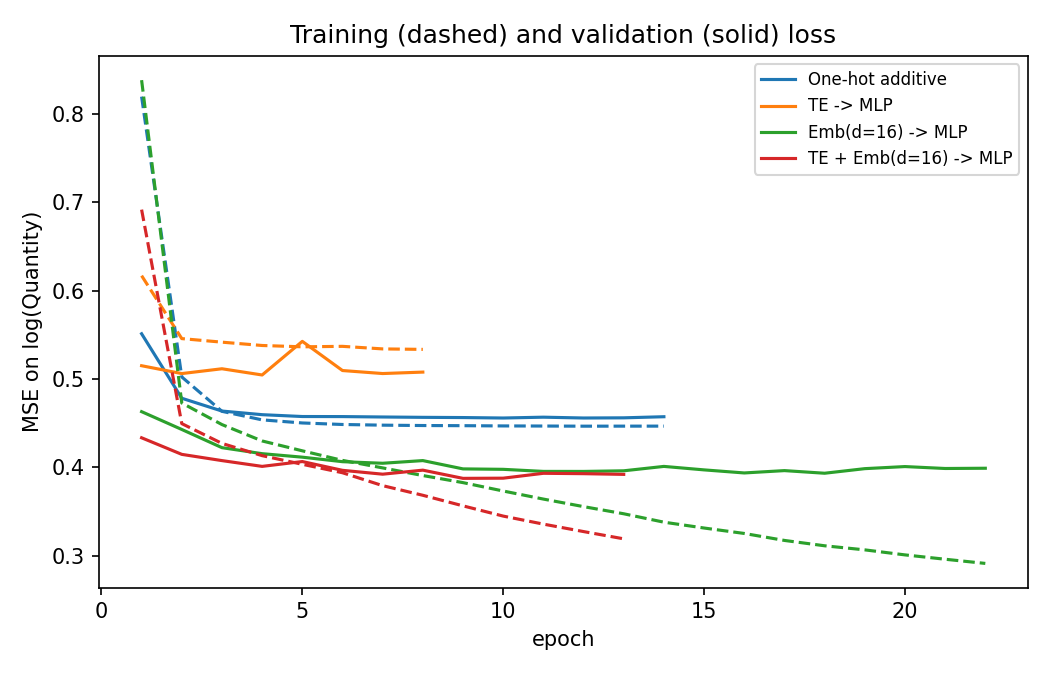
\includegraphics[width=0.66\textwidth]{problem2_training_curves.png}
\caption{Training (dashed) and validation (solid) MSE for the neural models.}
\label{fig:curves}
\end{figure}

%==========================================================================
\section*{(e) Intuition and supporting evidence}

\paragraph{What the embedding layer is.} Let $e_c\in\{0,1\}^K$ be the one-hot vector of level $c$.
An embedding lookup is a linear layer applied to the one-hot vector:
\[
 E[c] = E^\top e_c,\qquad E\in\R^{K\times d}.
\]
An embedding layer is therefore \emph{exactly} one-hot encoding followed by a trainable linear map
to $\R^d$, implemented as a lookup so the sparse matrix is never formed. Two special cases put
the other methods in the same framework:
\begin{itemize}
\item With $d=1$ and the two scalars \emph{summed} (no MLP), we get
$\hat t=b+a_{\text{item}}+b_{\text{cust}}$, which is precisely linear regression on one-hot
features. This is how I fit the one-hot baseline.
\item Target encoding is a $d=1$ ``embedding'' that is \emph{fixed in advance} to each level's
marginal mean of $t$, rather than learned for the task.
\end{itemize}
A learned $d=16$ embedding is a strict generalization of both. Each item and each customer gets a
16-dimensional vector of latent ``traits'', learned jointly with the MLP to minimize the loss.

\paragraph{Why it helps here.}
\begin{enumerate}
\item \textbf{Joint rather than marginal effects.} TE uses each feature's \emph{marginal} mean.
These means are confounded: a wholesale customer buys many bulk items, so the items they buy
have inflated marginal means, and vice versa. The model then double-counts. The one-hot
additive model estimates both effects \emph{jointly}, which is why it already beats
TE$\to$MLP ($0.673$ vs.\ $0.712$) even though it is linear. Embeddings are also learned jointly.
\item \textbf{One number per level is too little.} After target encoding, two items with the same
mean quantity are indistinguishable, even if one is bought in bulk by wholesalers and the other
in ones and twos by everybody. An MLP on $(\TE_{\text{item}},\TE_{\text{cust}})$ can only learn a
function of two scalars, and it gains little over the linear model on TE ($0.712$ vs.\ $0.728$).
\item \textbf{Interactions.} With $d$-dimensional vectors, the MLP can learn
\emph{customer$\times$item interactions}, e.g.\ ``this customer buys \emph{this kind} of item in
bulk''. That is a low-rank factorization of the $4{,}339\times3{,}665$ interaction table, in the
spirit of matrix factorization for recommender systems. One-hot features would need
$1.6\times10^7$ interaction columns for this, and TE cannot express it at all.
\end{enumerate}

\paragraph{Evidence on the test set.}

\emph{(i) Models use interactions only when given embeddings.} For each model I fitted the best
additive approximation $a_{\text{item}}+b_{\text{cust}}$ (by backfitting) to that model's own test
predictions. The fraction of prediction variance that is \emph{not} additive is:
\begin{center}
\begin{tabular}{lcccc}
\toprule
& One-hot additive & TE$\to$MLP & Emb$\to$MLP & TE+Emb$\to$MLP\\
\midrule
non-additive share of $\operatorname{Var}(\hat t)$ & 0.000 & 0.018 & 0.087 & 0.074\\
\bottomrule
\end{tabular}
\end{center}
The TE model is essentially additive. The embedding models put about 8--9\% of their prediction
variance into interaction effects, and they are also the models with the lowest test error.

\emph{(ii) Performance by how often a level is seen.} Tables~\ref{tab:item} and~\ref{tab:cust}
break down the test RMSE (log) by the number of training rows of the test row's item or customer.
\begin{table}[H]\centering
\begin{tabular}{lrccccc}
\toprule
train rows of item & $n_{\text{test}}$ & Global & One-hot add. & TE$\to$MLP & Emb$\to$MLP & TE+Emb\\
\midrule
0 (unseen)  & 53     & 1.277 & 0.720 & 0.820 & \textbf{0.701} & 0.736\\
1--10       & 929    & 1.276 & 0.749 & 0.847 & 0.747 & \textbf{0.745}\\
11--50      & 6{,}694  & 1.261 & 0.693 & 0.753 & 0.679 & \textbf{0.664}\\
51--200     & 25{,}416 & 1.196 & 0.669 & 0.701 & 0.624 & \textbf{0.613}\\
$>200$      & 26{,}598 & 1.203 & 0.669 & 0.707 & 0.614 & \textbf{0.612}\\
\bottomrule
\end{tabular}
\caption{Test RMSE (log) by frequency of the \texttt{StockCode} in training.}
\label{tab:item}
\end{table}
\begin{table}[H]\centering
\begin{tabular}{lrccccc}
\toprule
train rows of customer & $n_{\text{test}}$ & Global & One-hot add. & TE$\to$MLP & Emb$\to$MLP & TE+Emb\\
\midrule
0 (unseen)  & 21     & 2.206 & \textbf{1.142} & 1.833 & 1.282 & 1.149\\
1--10       & 1{,}298  & 1.338 & 0.711 & 0.935 & 0.704 & \textbf{0.679}\\
11--50      & 10{,}802 & 1.169 & 0.625 & 0.695 & 0.588 & \textbf{0.571}\\
51--200     & 24{,}519 & 1.150 & 0.632 & 0.666 & 0.584 & \textbf{0.577}\\
$>200$      & 23{,}050 & 1.275 & 0.732 & 0.750 & 0.684 & \textbf{0.682}\\
\bottomrule
\end{tabular}
\caption{Test RMSE (log) by frequency of the \texttt{CustomerID} in training.}
\label{tab:cust}
\end{table}
The embedding models win in every bucket with enough data. Their advantage over
TE is largest for \emph{rare} customers (1--10 rows: $0.935 \to 0.704$) and
shrinks as levels become more frequent (more than 200 rows: $0.750 \to 0.684$).
This points to over-shrinkage: with $m = 20$, a customer with $n_c \le 10$ rows
has $\lambda_c \le 1/3$, so its TE value is pulled most of the way to $\bar t$
(and further still for training rows, whose out-of-fold encodings use only
four-fifths of the data). The gap that remains for frequent levels reflects what
TE cannot represent at all: jointly estimated effects and interactions. Tuning
$m$ separately for each feature on the validation set would likely narrow the
first part of the gap. Part of this gap is also due to shrinkage: TE's deficit relative to the one-hot
additive model is largest for rare customers ($0.935$ vs.\ $0.711$ for 1--10
rows) and almost vanishes for frequent ones ($0.750$ vs.\ $0.732$ for more than
200 rows).

\emph{(iii) Pairs seen and not seen together.} 42\% of test rows are an (item, customer) pair that
also occurs in training. The embedding models improve on TE$\to$MLP for both seen pairs
($0.752\to0.662$) and \emph{unseen} pairs ($0.682\to0.586$). The gain on unseen pairs shows that
the improvement is not memorization of specific pairs. The model generalizes to new combinations
through the shared latent space, which is exactly what a factorization model should do.

\emph{(iv) Geometry of the learned embeddings.} Figure~\ref{fig:emb} shows the first two principal
components of the learned embeddings, coloured by each level's training mean of $t$. The first
principal component is strongly correlated with mean log quantity: $|\rho|=0.86$ for items and
$0.91$ for customers. So the main direction the network learns is essentially a target encoding
(``buys/is bought in large quantities''), learned from the loss rather than computed in advance.
The remaining directions (about half of the embedding variance) carry information that is
\emph{not} the mean, and that information is what the interactions use. Nearest neighbours also
look meaningful. For example, item \texttt{85099B} is closest to \texttt{23199}, \texttt{23202},
\texttt{23203} and \texttt{85099F}, a family of neighbouring codes (very likely variants of the same
product line) with similar typical order sizes. The embedding therefore groups related products,
even though the model was never told that their codes are related.

\begin{figure}[H]\centering
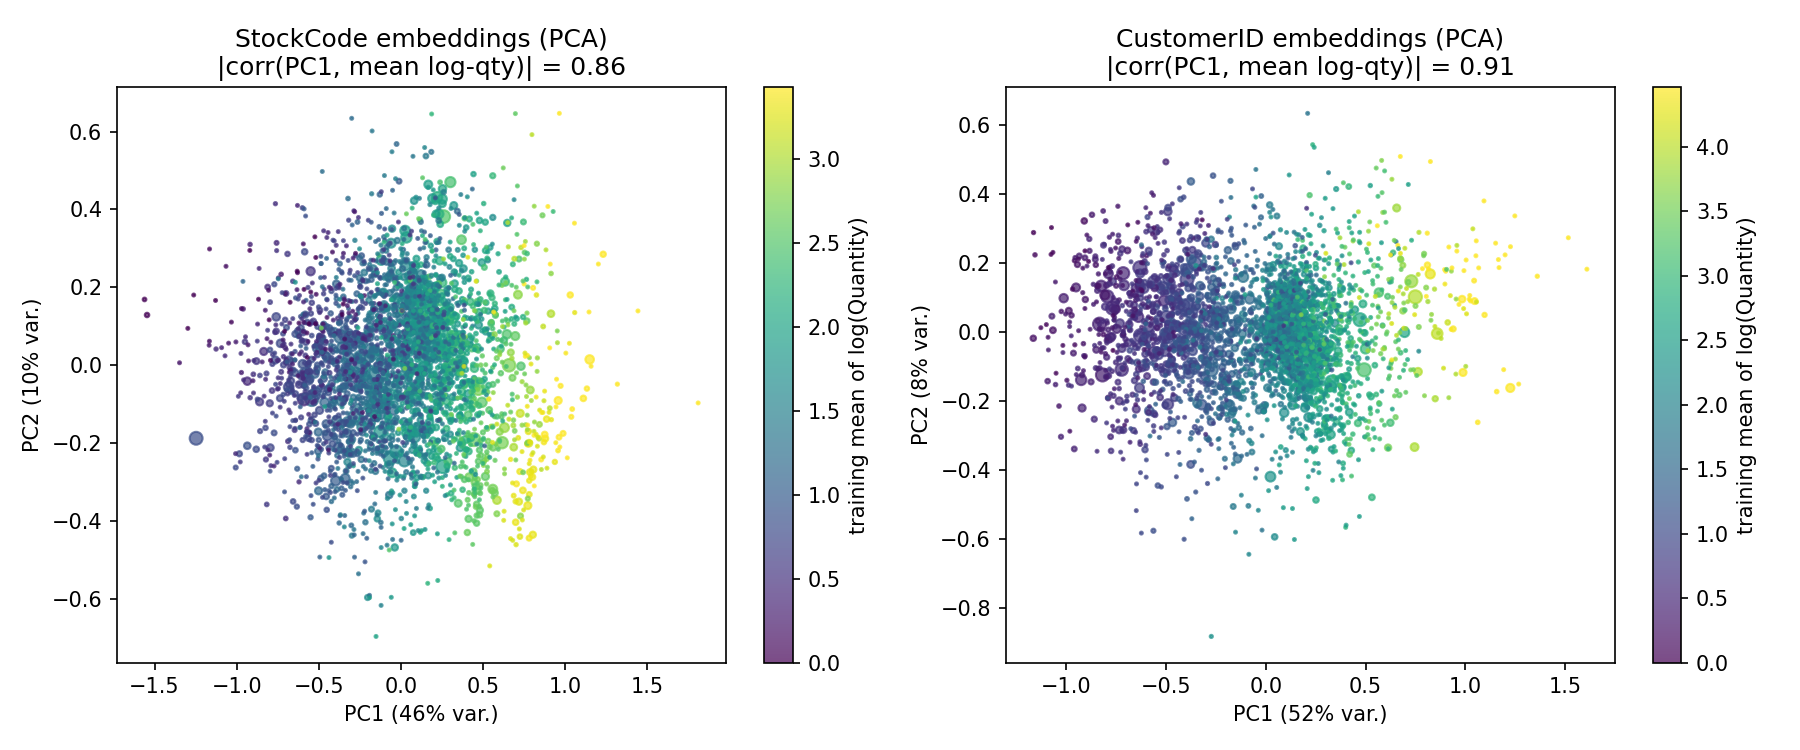
\includegraphics[width=\textwidth]{problem2_embeddings.png}
\caption{PCA of the learned $d=16$ embeddings (rows with $\ge3$ training transactions), coloured by
the training mean of $\log\texttt{Quantity}$; marker size $\propto$ frequency.}
\label{fig:emb}
\end{figure}

\paragraph{Summary.} Target encoding compresses each level into one fixed marginal statistic. It is
cheap and robust for rare levels, but it is confounded across features and cannot represent
interactions. Learned embeddings are one-hot encoding followed by a learned low-dimensional
projection. They estimate effects jointly, share statistical strength between similar levels, and
let the network learn low-rank item$\times$customer interactions, which gives the largest gain
(test MSE on the log scale: TE $0.507$, embeddings $0.395$, combined $0.386$). Combining the two
helps slightly, mainly for rare customers, because the shrunk TE value is a good summary where the
embedding has seen too little data.

\end{document}
